\section{Technology Stack}
\subsection{Front-end: React.js and Vite}
React.js handles the presentation layer of the online library, constructing interactive interfaces for book search, catalog browsing, and AI assistant chat interactions. Vite is employed as the build tool and dev server to provide fast startup, HMR support, and optimized production bundle compilation. On the client side, components handle rendering search results (incorporating keyword highlights and semantic matches), managing user state (caching, optimistic updates), and integrating the AI chat/assistant SDK (streaming responses, conversation state).
\begin{figure}[htbp]
    \centering
    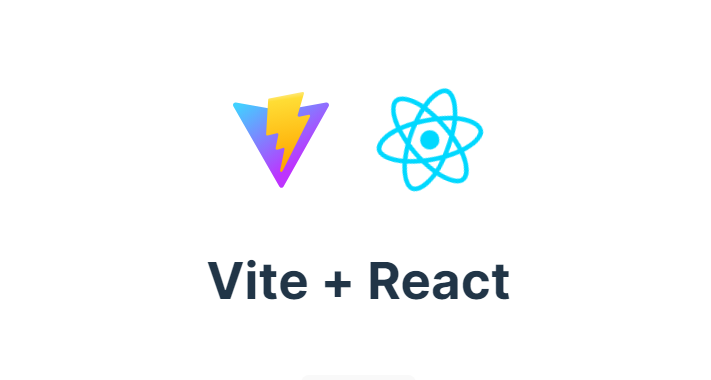
\includegraphics[width=0.4\textwidth]{Images/react_vite.png}
\end{figure}

\subsection{Back-end: Node.js and Express}
Node.js + Express provides the core REST API for book catalog management, user accounts, and session administration. The server orchestrates request routing, authentication, RBAC authorization, PostgreSQL transactions via Prisma, and delegates AI workloads (embedding generation, summarization, RAG queries) to dedicated AI services. It exposes standardized endpoints for search, recommendations, and integration webhooks (e.g., metadata enrichment from Open Library).
\begin{figure}[htbp]
    \centering
    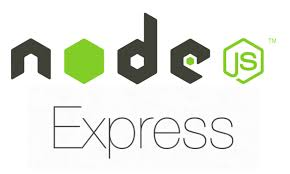
\includegraphics[width=0.4\textwidth]{Images/node_express.jpg}
\end{figure}

\subsection{Dedicated AI Microservice: Python and FastAPI}
A decoupled microservice implemented in Python + FastAPI leverages NLP and Machine Learning frameworks (transformers, sentence-transformers, LLM provider client SDKs). Its primary responsibilities include embedding vector generation, document summarization, RAG-based question answering, and prompt engineering pipelines (chunking, reranking). FastAPI is ideal for low-latency concurrent endpoints and seamlessly scales based on workload demands.
\begin{figure}[htbp]
    \centering
    
\includegraphics[width=0.4\textwidth]{Images/fastapi.png}
\end{figure}

\subsection{ORM: Prisma}
Prisma (TypeScript) is used to define database schemas, generate type-safe query clients, and manage PostgreSQL migrations. Prisma maintains end-to-end type safety between the Node application and the database layer, simplifying queries related to loans, transaction logs, and catalog metadata while providing ACID transaction support for data consistency.
\begin{figure}[htbp]
    \centering
    
\includegraphics[width=0.4\textwidth]{Images/prisma.png}
\end{figure}

\subsection{Relational Database: PostgreSQL}
PostgreSQL serves as the primary relational store for book records, user profiles, loan transactions, and system metadata. Key advantages include strict ACID compliance for loan-return workflows, advanced JSONB support for flexible metadata, full-text keyword indexing, and horizontal scalability via replication and partitioning.
\begin{figure}[htbp]
    \centering
    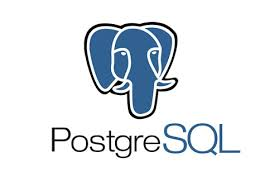
\includegraphics[width=0.4\textwidth]{Images/postgresql.jpg}
\end{figure}

\subsection{Vector Store and Embeddings: pgvector}
Text embeddings for book contents (full texts, summaries) are stored in `pgvector` (a vector extension for PostgreSQL) or a dedicated vector database. The vector store performs nearest-neighbor searches (cosine similarity) to power semantic search, contextual retrieval for RAG pipelines, and "similar books" recommendation features, mapping vector outputs directly to source document IDs.

\subsection{AI / LLM Capabilities: Embeddings, RAG, Summarization, and Chatbot}
The system integrates Large Language Models (LLMs) across multiple modules: embedding generation for semantic search, Retrieval-Augmented Generation (RAG) for Q\&A based on library documents, automatic chapter/abstract summarization for previews, and interactive chatbot assistants. The architecture incorporates controlled prompt templates, embedding caching, and attribution mechanisms for source citation.
\begin{figure}[htbp]
    \centering
    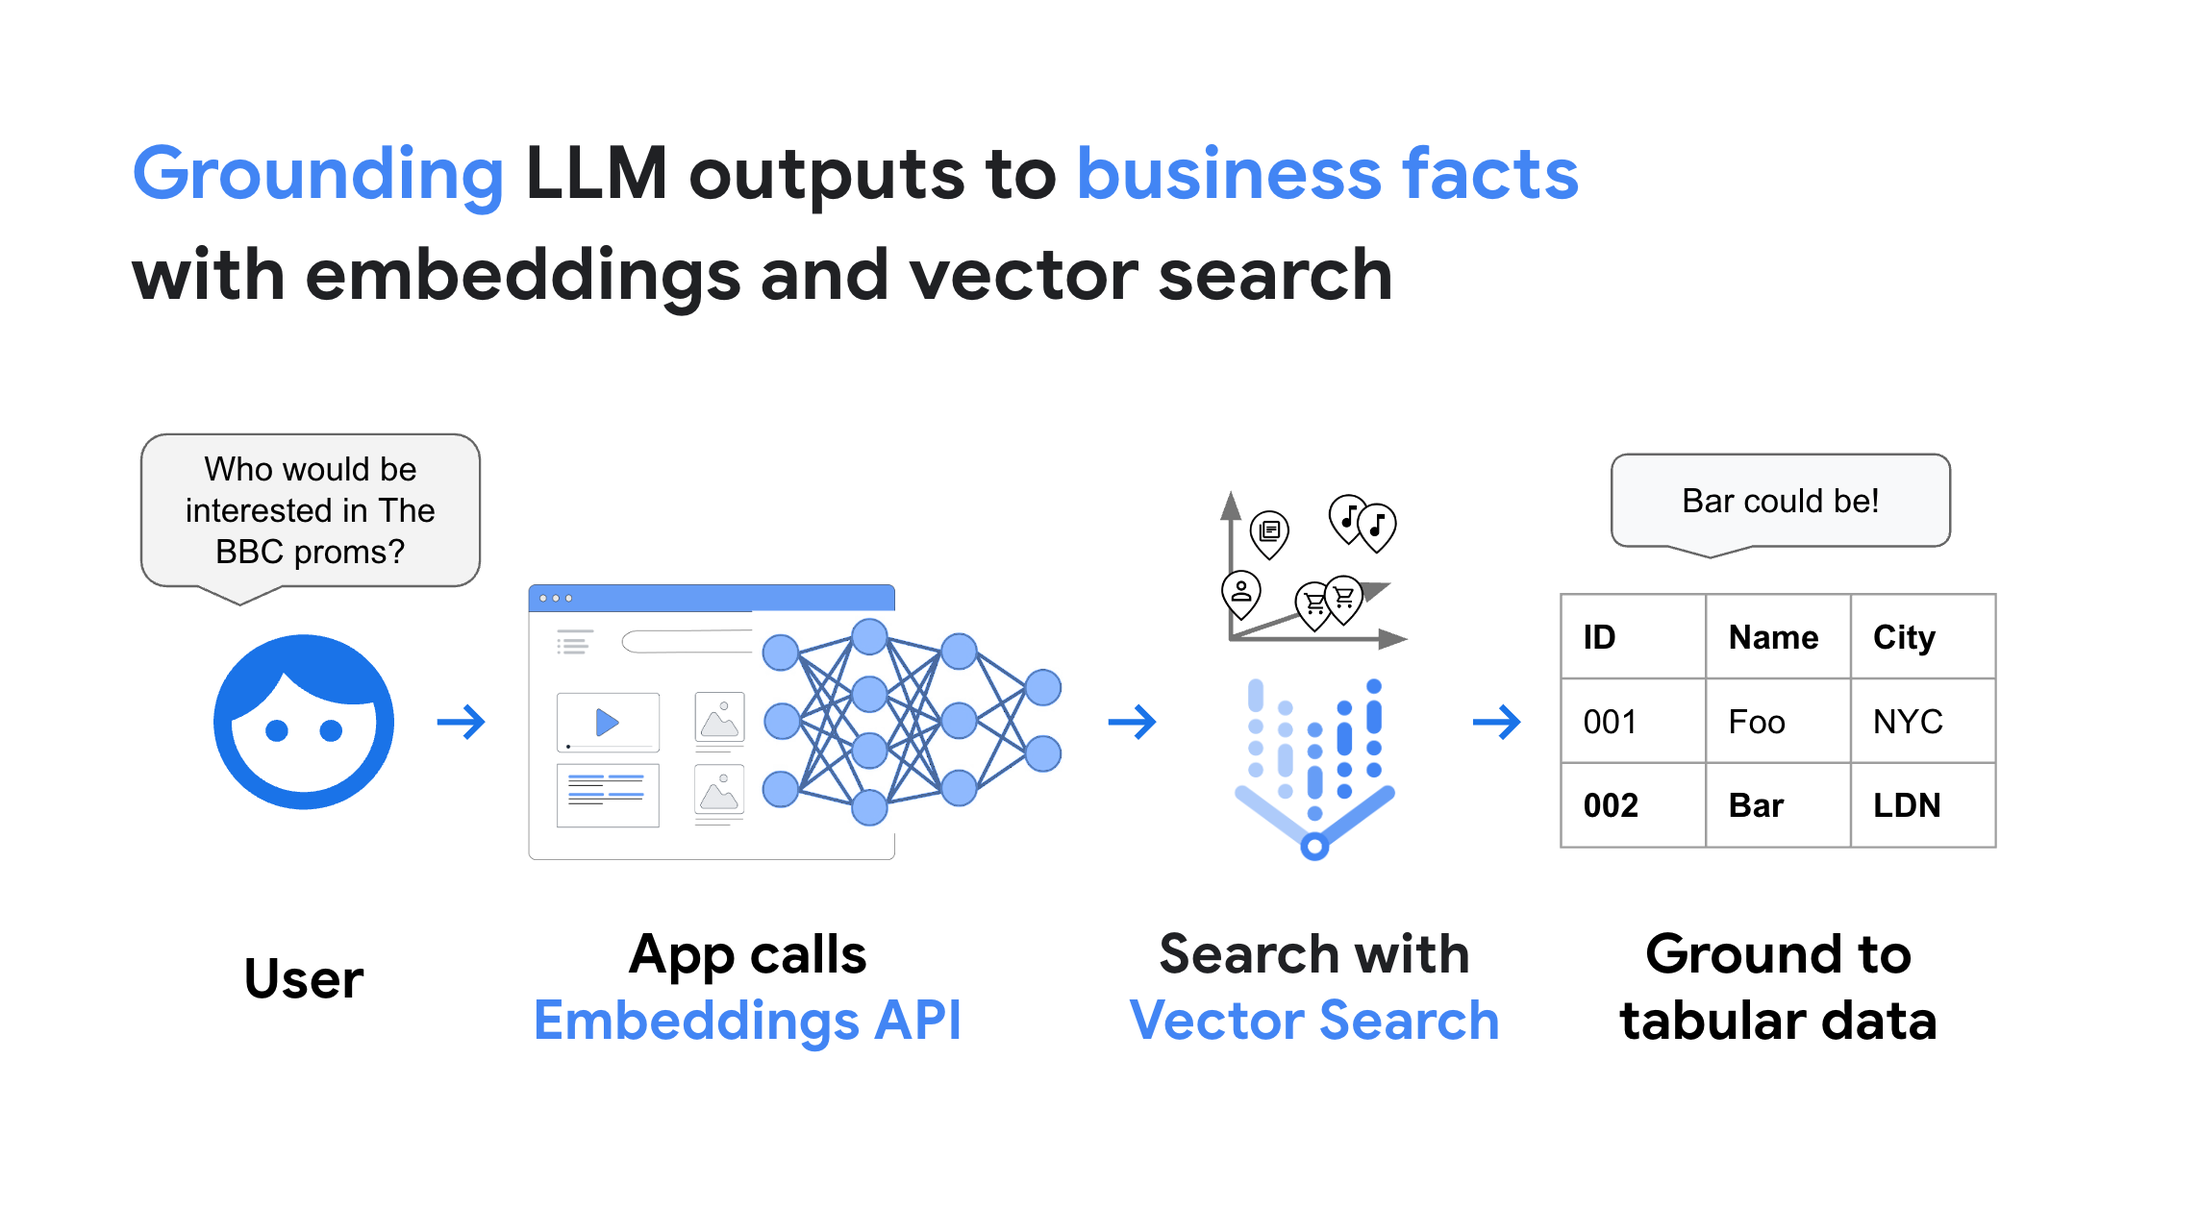
\includegraphics[width=0.5\textwidth]{Images/EmbeddingsAPI.png}
\end{figure}

\subsection{Hybrid Search Strategy}
A hybrid search strategy combines: 1) full-text keyword search on PostgreSQL for exact metadata matching; and 2) vector similarity search via pgvector for semantic retrieval and contextual matching. Results are merged and reranked (based on relevance scores, popularity, and user context) before returning to the client interface.

\subsection{Security and Authentication: JWT, RBAC, and OTP}
The system utilizes JSON Web Tokens (JWT) for session management and refresh tokens for secure persistence. Role-Based Access Control (RBAC) enforces granular permissions (Admin, Librarian, Reader) verified at API gateways and endpoints. One-Time Passwords (OTP via email/SMS) secure multi-factor authentication for sensitive operations. Additional measures include HTTPS/TLS encryption, rate limiting, and comprehensive audit logging.

\subsection{External Integrations: Open Library, Google Books, and Nodemailer}
The Open Library and Google Books APIs automate metadata, cover image, and publishing data fetching via ISBN lookup. An automated ETL pipeline periodically syncs catalog data. `Nodemailer` handles transactional notifications (loan due reminders, password resets, system alerts) with dynamic HTML templates and delivery logging.
\begin{figure}[htbp]
    \centering
    
\includegraphics[width=0.3\textwidth]{Images/Google-play-book-icon.png}
\end{figure}